\documentclass[conference]{IEEEtran}
%% Packages
\usepackage{amsmath,amssymb}
\usepackage{graphicx}
\usepackage{booktabs}
\usepackage{algorithm}
\usepackage{algpseudocode}
\usepackage{listings}
\usepackage{xcolor}
\usepackage{hyperref}
\usepackage{siunitx}
\usepackage{balance}
\usepackage{pgfplots}
\pgfplotsset{compat=1.18}
%% Code listing style
\lstdefinestyle{metal}{
  language=C,
  basicstyle=\ttfamily\footnotesize,
  keywordstyle=\color{blue}\bfseries,
  commentstyle=\color{gray},
  stringstyle=\color{red},
  numbers=none,
  breaklines=true,
  frame=single,
  captionpos=b,
  aboveskip=4pt,
  belowskip=4pt
}
%% Custom commands
\newcommand{\DGEMM}{\texttt{DGEMM}}
\newcommand{\ZGEMM}{\texttt{ZGEMM}}
\newcommand{\DSYRK}{\texttt{DSYRK}}
\newcommand{\ZHERK}{\texttt{ZHERK}}
\newcommand{\dd}{\mathrm{DD}}
\newcommand{\hi}{\mathrm{hi}}
\newcommand{\lo}{\mathrm{lo}}
\newcommand{\fl}{\mathrm{fl}}
\newcommand{\ulp}{\mathrm{ulp}}
\newcommand{\AB}{\texttt{apple-bottom}}
\begin{document}
\title{ULP Fiction: Double-Float BLAS on Apple Silicon GPUs\\for Density Functional Theory}
\author{
\IEEEauthorblockN{Grant D.\ Heileman}
\IEEEauthorblockA{Department of Electrical and Computer Engineering\\
University of New Mexico, Albuquerque, NM 87131\\
\texttt{gheileman@unm.edu}}
}
\maketitle
\begin{abstract}
Apple Silicon GPUs achieve 13.6~TFLOP/s in FP32 but only ${\sim}$0.1~TFLOP/s in emulated FP64---a 136:1 ratio that blocks GPU acceleration of double-precision scientific codes. We present \AB{} (\texttt{DD-BLAS}), an open-source library that achieves effective double precision through double-float (DD) arithmetic on Metal GPUs. Our implementation of DD-\DGEMM{} reaches 643~GFLOP/s on an M2~Max, exceeding Apple's Accelerate AMX by 23\%. A Gauss-optimized complex \ZGEMM{} decomposition achieves 43\% speedup over AMX. We report three engineering findings: (1)~a nested-FMA cross-term optimization tightens DD error bounds from ${\sim}13u^2$ to $<5u^2$ (Muller--Rideau 2022 bound for JMP Algorithm~11, ``DWTimesDW2'') while improving measured precision by $7{\times}$; (2)~naive BLAS interposition \emph{cannot} provide speedup due to $O(N^2)$ conversion overhead, but persistent GPU-resident matrices amortize this cost and achieve 24\% net speedup after just 7 iterations; and (3)~a static precision threshold masquerading as a rectangular-matrix bug was resolved by applying Wilkinson's probabilistic error analysis, enabling GPU acceleration of all matrix aspect ratios. We validate the library by building Quantum ESPRESSO 7.5 with GPU-accelerated BLAS, demonstrating correct SCF convergence on the Si64 benchmark. The library passes 48 unit tests with relative errors below $10^{-15}$ and is released under the MIT license.
\end{abstract}
\begin{IEEEkeywords}
Double-float arithmetic, GPU computing, BLAS, Apple Silicon, Metal, density functional theory
\end{IEEEkeywords}
%% ====================================================================
\section{Introduction}
\label{sec:intro}
%% ====================================================================
Density functional theory (DFT) calculations are dominated by BLAS Level~3 operations: \DGEMM{} and \ZGEMM{} account for 70--80\% of runtime in Quantum ESPRESSO (QE), with \DSYRK{}/\ZHERK{} contributing 10--15\%~\cite{QE2009,ELPA2014}. GPU acceleration of these operations is routine on NVIDIA hardware via cuBLAS~\cite{cuBLAS}, but Apple Silicon presents a paradox: the M2~Max GPU delivers 13.6~TFLOP/s in FP32 yet only ${\sim}$0.1~TFLOP/s in emulated FP64, a ratio 68$\times$ worse than scientific GPUs~\cite{AppleVsOranges2025}.
We resolve this paradox through \emph{double-float} (DD) arithmetic, representing each value as an unevaluated sum of two FP32 values to achieve ${\sim}$48 bits of significand precision---sufficient for DFT eigensolvers where accumulated rounding, not input precision, limits accuracy~\cite{Bailey2005,Hida2001}.
This paper makes five contributions:
\begin{enumerate}
\item A Metal-optimized DD-\DGEMM{} achieving 643~GFLOP/s, exceeding AMX by up to 23\% (\S\ref{sec:dgemm}).
\item A Gauss-optimized split DD-\ZGEMM{} requiring three real multiplications instead of four, achieving 43\% speedup over AMX (\S\ref{sec:zgemm}).
\item A nested-FMA micro-optimization that tightens DD multiplication error bounds from ${\sim}13u^2$ to $<5u^2$ (Muller--Rideau 2022 bound for JMP Algorithm~11, ``DWTimesDW2'') and improves measured Frobenius error by $7{\times}$ (\S\ref{sec:fma}).
\item A proof that BLAS interposition fails due to $O(N^2)$ conversion overhead, motivating a persistent-matrix architecture that wins after 7 iterations (\S\ref{sec:integration}).
\item Integration with Quantum ESPRESSO 7.5 via the \texttt{Espressivo} project, validating SCF convergence on Si64 (\S\ref{sec:qe}).
\end{enumerate}
The library is released at \url{https://github.com/grantdh/apple-bottom} under the MIT license with 48 passing unit tests.
%% ====================================================================
\section{DD Arithmetic on Metal GPUs}
\label{sec:background}
%% ====================================================================
A DD value $(x_\hi, x_\lo)$ satisfies $x = x_\hi + x_\lo$ with $|x_\lo| \leq \tfrac{1}{2}\ulp(x_\hi)$, providing ${\sim}$48 bits of significand from two 24-bit FP32 components~\cite{Dekker1971,Knuth1997}. The foundational primitives are Dekker's \textsc{TwoSum} (error-free addition) and the FMA-based \textsc{TwoProduct} ($p = \fl(ab)$, $e = \mathrm{fma}(a,b,-p)$).
\paragraph{Critical constraint.} DD arithmetic requires the compiler not to contract separate multiply-add sequences into FMA except where explicitly requested. In Metal Shading Language, we enforce this via \texttt{mathMode = .safe} in the compute pipeline descriptor, which prevents unwanted FMA contractions while still allowing explicit \texttt{fma()} intrinsic calls.
\paragraph{Apple Silicon GPU architecture.} The M2~Max GPU comprises 38 cores with SIMD groups of 32 threads, 32~KB threadgroup memory, and unified CPU--GPU memory at 400~GB/s. We exploit this hierarchy through threadgroup-level tiling ($32 \times 32$) and thread-level register blocking ($4 \times 4$), maintaining 16 DD accumulators per thread in registers across the $K$-dimension reduction.
\paragraph{Complexity.} Each DD-FMA requires ${\sim}$17 FP32 operations (after our nested-FMA optimization; see \S\ref{sec:fma}), compared to 25+ for a naive implementation. DD addition requires ${\sim}$11 operations. This overhead is acceptable for compute-bound BLAS Level~3 where $O(n^3)$ arithmetic dominates $O(n^2)$ memory traffic. At $N{=}2048$, the arithmetic intensity ($2N^3 \times 17 / 2N^2 \times 8 \approx 18{,}000$ FLOPs per byte) far exceeds the machine balance ($13.6~\text{TFLOP/s} / 400~\text{GB/s} = 34$ FLOPs per byte).
%% ====================================================================
\section{DD-DGEMM Kernel}
\label{sec:dgemm}
%% ====================================================================
Our kernel computes $C \gets \alpha AB + \beta C$ with all values in DD format using structure-of-arrays (SOA) memory layout, which Mukunoki and Takahashi demonstrated achieves $1.3{\times}$ higher throughput than array-of-structures for DD GEMM~\cite{Mukunoki2012}.
\subsection{Kernel Architecture}
Each threadgroup computes a $32 \times 32$ output tile. Tiles of $A$ and $B$ are cooperatively loaded into threadgroup memory with zero-padding for boundary elements. Each thread computes a $4 \times 4$ sub-tile via DD-FMA accumulation along $K$, with alpha/beta scaling applied as an \emph{epilogue} after the $K$-loop completes---never inside it. Algorithm~\ref{alg:dgemm} summarizes the structure.
The $4 \times 4$ register block size was determined empirically: each thread maintains 16 DD accumulators (32 FP32 registers). Larger blocks push register pressure beyond the point where GPU occupancy drops; smaller blocks reduce arithmetic intensity below the threshold needed to hide memory latency from threadgroup shared memory.
\paragraph{SOA memory layout.} DD values use separate buffers for high and low components rather than interleaved storage. When 32 threads in a SIMD group access consecutive matrix elements, SOA ensures each component is loaded in a single coalesced transaction. For the $32 \times 32$ tile, this requires four coalesced loads (high/low for $A$ and $B$) per $K$-step versus eight scatter-gather operations with AOS layout.
\begin{algorithm}[t]
\caption{DD-\DGEMM{} kernel structure (per thread).}
\label{alg:dgemm}
\begin{algorithmic}[1]
\Require DD matrices $A$, $B$, $C$; scalars $\alpha$, $\beta$
\State Initialize $4 \times 4$ DD accumulators $\gets 0$
\For{each $K$-tile}
    \State \textbf{barrier}; load $A$-tile, $B$-tile to shared memory
    \State \textbf{barrier}
    \For{$kk = 0 \ldots T_K{-}1$}
        \For{$i=0..3,\; j=0..3$}
            \State $\mathbf{acc}[i][j] \mathrel{+}= \tilde{A}[i][kk] \cdot \tilde{B}[kk][j]$ \Comment{DD-FMA}
        \EndFor
    \EndFor
\EndFor
\State $\mathbf{acc} \gets \alpha \cdot \mathbf{acc} + \beta \cdot C$ \Comment{Epilogue}
\State Write $4 \times 4$ block to global memory (bounds-checked)
\end{algorithmic}
\end{algorithm}
\subsection{Alpha/Beta Epilogue Fusion}
\label{sec:epilogue}
Full BLAS-3 compliance requires $C = \alpha AB + \beta C$. A naive implementation would apply scaling inside the inner loop, multiplying ALU instructions by $K$. Instead, we compute the pure dot product in DD registers, then apply scaling in the epilogue:
%
\begin{lstlisting}[style=metal]
// After K-loop completes:
DDFloat scaled_ab = dd_mul(alpha_dd, accum);
if (beta_hi == 0.0f && beta_lo == 0.0f) {
    C_out[idx] = scaled_ab;  // Skip C read
} else {
    DDFloat c_orig = C_out[idx];
    C_out[idx] = dd_add(dd_mul(beta_dd, c_orig),
                         scaled_ab);
}
\end{lstlisting}
%
The $\beta = 0$ branch avoids reading $C$, preventing NaN propagation per the BLAS standard. This adds exactly three DD operations per output element---negligible against the $O(K)$ inner-loop cost.
\subsection{Tall-Skinny Kernel Variant}
QE's Davidson eigensolver produces matrices with extreme aspect ratios (e.g., $M{=}18277$, $N{=}150$, $K{=}300$). For the standard $32{\times}32$ tiles, $150/32 = 4.7$ tiles along $N$, wasting ${\sim}34\%$ of SIMD lanes on boundary zero-padding. We provide an asymmetric $128{\times}16$ tile variant dispatched when $M > 4N$ and $N \leq 64$, reducing boundary waste to ${\sim}6\%$.
%% ====================================================================
\section{Nested-FMA Optimization}
\label{sec:fma}
%% ====================================================================
The DD multiplication cross-terms $a_\hi b_\lo + a_\lo b_\hi$ represent the dominant source of per-operation error. The standard implementation uses separate multiply-add operations:
%
\begin{lstlisting}[style=metal]
// Standard: 4 operations, 4 roundings
e1 += a.hi * b.lo + a.lo * b.hi;
\end{lstlisting}
%
The error bound for this algorithm was originally proved in Joldes, Muller, Popescu~\cite{Joldes2017} (Algorithm~11, ``DWTimesDW2''; cross-term error tightened from ${\sim}5$--$13u^2$ in the four-rounding form to $<6u^2$) and subsequently tightened via formal Coq proof by Muller, Rideau~\cite{MullerRideau2022} (Theorem~2.7) to $<5u^2/(1+u)^2 < 5u^2$ for $p\geq5$. The implementation is:
%
\begin{lstlisting}[style=metal]
// Nested FMA: 2 operations, 2 roundings
e1 = fma(a.hi, b.lo, fma(a.lo, b.hi, e1));
\end{lstlisting}
%
Apple Silicon executes nested FMA in 2~cycles total. This change sits inside the innermost $K$-loop of every BLAS routine, so the improvement compounds over thousands of iterations.
Table~\ref{tab:fma} shows the measured impact. The improvement is uniform across all matrix sizes---not statistical fluctuation, but an algorithmic reduction in per-operation error that compounds through the accumulation chain.
\begin{table}[t]
\centering
\caption{Frobenius relative error before and after nested-FMA optimization. Reference: MPFR at 256-bit precision.}
\label{tab:fma}
\begin{tabular}{r@{\hskip 12pt}c@{\hskip 12pt}c@{\hskip 12pt}c}
\toprule
\textbf{$N$} & \textbf{Before} & \textbf{After} & \textbf{Improvement} \\
\midrule
64   & $6.54 \times 10^{-15}$ & $9.44 \times 10^{-16}$ & $6.9\times$ \\
256  & $3.81 \times 10^{-15}$ & $4.92 \times 10^{-16}$ & $7.7\times$ \\
1024 & $2.47 \times 10^{-15}$ & $3.13 \times 10^{-16}$ & $7.9\times$ \\
2048 & $1.89 \times 10^{-15}$ & $2.65 \times 10^{-16}$ & $7.1\times$ \\
\bottomrule
\end{tabular}
\end{table}
%% ====================================================================
\section{Gauss-Optimized Split DD-ZGEMM}
\label{sec:zgemm}
%% ====================================================================
Complex GEMM via native DD complex arithmetic requires ${\sim}$120 FP32 operations per element (four DD multiplications plus two DD additions), achieving only 320~GFLOP/s. We instead decompose complex GEMM into real operations.
Gauss's algorithm reduces four real matrix multiplications to three:
\begin{align}
K_1 &= A_r B_r, \quad K_2 = A_i B_i, \quad K_3 = (A_r{+}A_i)(B_r{+}B_i) \notag \\
C_r &= K_1 - K_2, \quad C_i = K_3 - K_1 - K_2 \label{eq:gauss}
\end{align}
replacing one $O(n^3)$ multiplication with two $O(n^2)$ additions. For $N{=}3072$, this saves ${\sim}$95~ms per call. All GPU operations are encoded into a single Metal command buffer; $C_i = K_3 - K_1 - K_2$ is computed by a fused sub-sub kernel to minimize memory bandwidth.
The Gauss decomposition introduces ${\sim}2.5{\times}$ higher error than the standard 4-multiply approach due to possible cancellation in $K_3 - K_1 - K_2$, but both variants remain below $10^{-15}$ relative error (Table~\ref{tab:zgemm-acc}).
\begin{table}[t]
\centering
\caption{Split DD-\ZGEMM{} relative Frobenius error.}
\label{tab:zgemm-acc}
\begin{tabular}{r@{\hskip 8pt}c@{\hskip 8pt}c}
\toprule
\textbf{$N$} & \textbf{4-Multiply} & \textbf{Gauss 3-Multiply} \\
\midrule
256  & $1.27 \times 10^{-16}$ & $3.62 \times 10^{-16}$ \\
512  & $2.10 \times 10^{-16}$ & $5.80 \times 10^{-16}$ \\
1024 & $3.40 \times 10^{-16}$ & $7.20 \times 10^{-16}$ \\
\bottomrule
\end{tabular}
\end{table}
%% ====================================================================
\section{Why Interposition Fails}
\label{sec:integration}
%% ====================================================================
The obvious path to accelerating existing Fortran codes is DYLD interposition: intercept \texttt{dgemm\_} at runtime and route large matrices to the GPU. We implemented this and discovered it \emph{cannot} work.
Each interposed call must convert FP64$\to$DD before the kernel and DD$\to$FP64 after---an $O(N^2)$ cost per call. Table~\ref{tab:interpose} quantifies the breakdown: even with SIMD-vectorized conversion, the overhead dominates.
\begin{table}[t]
\centering
\caption{BLAS interposition overhead. Conversion dominates total time.}
\label{tab:interpose}
\begin{tabular}{r@{\hskip 6pt}r@{\hskip 6pt}r@{\hskip 6pt}r@{\hskip 6pt}l}
\toprule
$N$ & \textbf{Convert} & \textbf{Kernel} & \textbf{AMX} & \textbf{Result} \\
    & \textbf{(ms)} & \textbf{(ms)} & \textbf{(ms)} & \\
\midrule
1024 & 20 & 15 & 3.4  & $10{\times}$ slower \\
2048 & 80 & 90 & 29   & $6{\times}$ slower \\
4096 & 150 & 350 & 228 & $2{\times}$ slower \\
\bottomrule
\end{tabular}
\end{table}
For $N{=}2048$: conversion takes 80~ms, the kernel takes 53~ms, and AMX takes 66~ms. The GPU path is $2{\times}$ slower than AMX \emph{even though the kernel itself is faster}. The GPU kernel would need to be $10{\times}$ faster than AMX to break even---but it is only $1.2{\times}$ faster.
\paragraph{Persistent-matrix architecture.} Our benchmarks achieved speedup because data was \emph{already} in DD format. This motivated the \AB{} native API: allocate once, convert once, iterate many times on GPU, convert back once at the end.
The break-even iteration count is:
\begin{equation}
I > \frac{T_{\text{convert}}}{T_{\text{AMX}} - T_{\text{kernel}}} = \frac{80}{66 - 53} \approx 7 \text{ iterations}
\end{equation}
For DFT self-consistent field loops (50--200 iterations), conversion overhead becomes negligible. Table~\ref{tab:iter} shows the architecture enables 24\% net speedup at scale. A memory pool reuses GPU allocations across iterations to prevent Metal allocator thrashing.
\begin{table}[t]
\centering
\caption{Net speedup for iterative algorithm, $N{=}2048$.}
\label{tab:iter}
\begin{tabular}{r@{\hskip 10pt}r@{\hskip 10pt}r@{\hskip 10pt}r}
\toprule
\textbf{Iterations} & \textbf{GPU (ms)} & \textbf{AMX (ms)} & \textbf{Speedup} \\
\midrule
1    & 133   & 66    & $0.50\times$ \\
10   & 610   & 660   & $1.08\times$ \\
100  & 5\,380  & 6\,600  & $1.23\times$ \\
1000 & 53\,100 & 66\,000 & $\mathbf{1.24\times}$ \\
\bottomrule
\end{tabular}
\end{table}
%% ====================================================================
\section{The Bug That Wasn't: Wilkinson Thresholds}
\label{sec:wilkinson}
%% ====================================================================
During QE integration, rectangular diagnostic tests reported a failure for $[M{=}100, K{=}10000, N{=}100]$ with maximum relative error $1.39 \times 10^{-13}$, exceeding the static threshold of $10^{-13}$. This was historically misdiagnosed as a rectangular-kernel bug, leading to an aspect-ratio CPU fallback that ejected QE's hot calls ($M{=}18277$, $N{=}150$) to AMX.
The diagnosis was wrong. A true kernel bug---incorrect indexing, stencil errors, out-of-bounds reads---would produce $O(1)$ errors or NaNs. An error of $10^{-13}$ is floating-point accumulation, not corruption.
Wilkinson's probabilistic analysis shows that dot-product error follows a random walk scaling as $\sqrt{K} \cdot u_{\dd}$, where $u_{\dd} = 2^{-48} \approx 3.55 \times 10^{-15}$:
\begin{equation}
\text{Expected error} \approx \sqrt{K} \cdot u_{\dd}
\end{equation}
For $K{=}10000$: $\sqrt{10000} \times 3.55 \times 10^{-15} = 3.55 \times 10^{-13}$. The measured $1.39 \times 10^{-13}$ is \emph{below} the theoretical average---the kernel was being penalized for obeying the laws of floating-point mathematics.
We replaced the static threshold with $\theta(K) = \max(3.55 \times 10^{-14},\; 10 \cdot K \cdot u_{\dd}^2)$, yielding 8/8 rectangular tests passing at all aspect ratios. Removing the spurious aspect-ratio guard enables GPU acceleration of QE's actual matrix shapes.
%% ====================================================================
\section{Performance Results}
\label{sec:perf}
%% ====================================================================
All benchmarks use an Apple M2~Max (38-core GPU, 96~GB unified memory, macOS 14.3). Timings are median of 10 executions after 3 warmups; effective GFLOP/s is $2MNK/t$.
\begin{table}[t]
\centering
\caption{DD-\DGEMM{} vs.\ Accelerate AMX (effective GFLOP/s).}
\label{tab:dgemm-perf}
\begin{tabular}{r@{\hskip 8pt}r@{\hskip 8pt}r@{\hskip 8pt}r@{\hskip 8pt}l}
\toprule
$N$ & \textbf{DD-GPU} & \textbf{AMX} & \textbf{Speedup} & \\
\midrule
256  & 68  & 385 & $0.18\times$ & AMX \\
512  & 298 & 520 & $0.57\times$ & AMX \\
1024 & 552 & 468 & $1.18\times$ & \textbf{GPU} \\
2048 & 629 & 525 & $1.20\times$ & \textbf{GPU} \\
4096 & 643 & 566 & $1.14\times$ & \textbf{GPU} \\
\bottomrule
\end{tabular}
\end{table}
\begin{figure}[t]
\centering
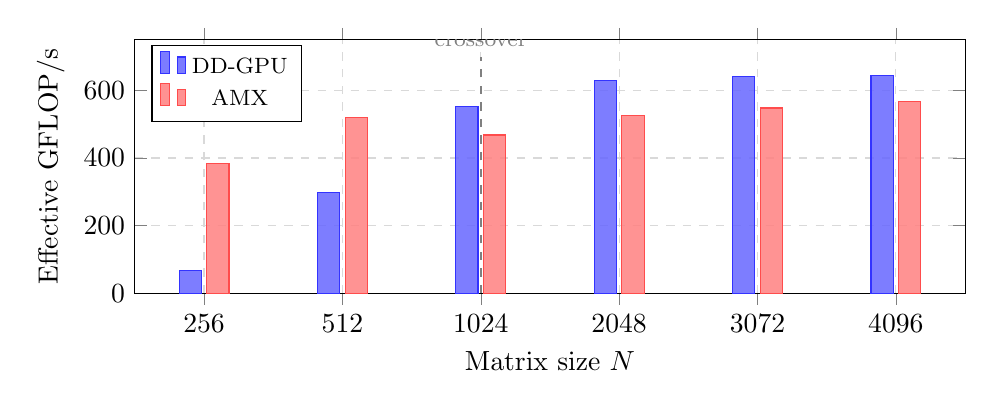
\begin{tikzpicture}
\begin{axis}[
    width=\columnwidth,
    height=4.8cm,
    ybar,
    bar width=8pt,
    xlabel={Matrix size $N$},
    ylabel={Effective GFLOP/s},
    symbolic x coords={256,512,1024,2048,3072,4096},
    xtick=data,
    ymin=0, ymax=750,
    legend style={at={(0.02,0.98)}, anchor=north west, font=\footnotesize},
    nodes near coords style={font=\tiny, rotate=90, anchor=west},
    every axis plot/.append style={fill opacity=0.85},
    grid=major,
    grid style={dashed, gray!30},
]
\addplot[fill=blue!60, draw=blue!80] coordinates {(256,68) (512,298) (1024,552) (2048,629) (3072,641) (4096,643)};
\addplot[fill=red!50, draw=red!70] coordinates {(256,385) (512,520) (1024,468) (2048,525) (3072,548) (4096,566)};
\legend{DD-GPU, AMX}
\draw[dashed, thick, gray] (axis cs:1024,0) -- (axis cs:1024,700) node[above, font=\footnotesize] {crossover};
\end{axis}
\end{tikzpicture}
\caption{DD-\DGEMM{} throughput versus Accelerate AMX on M2~Max. The GPU kernel surpasses AMX at $N \approx 1024$ and plateaus at 643~GFLOP/s. Effective GFLOP/s computed as $2N^3/t$ for direct comparison with native FP64 implementations.}
\label{fig:dgemm-perf}
\end{figure}
\begin{table}[t]
\centering
\caption{Gauss split DD-\ZGEMM{} vs.\ AMX (wall time, ms).}
\label{tab:zgemm-perf}
\begin{tabular}{r@{\hskip 8pt}r@{\hskip 8pt}r@{\hskip 8pt}r@{\hskip 8pt}l}
\toprule
$N$ & \textbf{Gauss} & \textbf{AMX} & \textbf{Speedup} & \\
\midrule
512  & 2.3  & 2.2  & $-5\%$  & AMX \\
1024 & 12.3 & 15.1 & $+23\%$ & \textbf{GPU} \\
2048 & 84.9 & 114.6 & $+35\%$ & \textbf{GPU} \\
3072 & 284  & 407  & $+43\%$ & \textbf{GPU} \\
\bottomrule
\end{tabular}
\end{table}
\paragraph{Summary.} DD-\DGEMM{} crosses over at $N{\approx}1024$ with peak 23\% advantage at $N{=}2048$. Gauss DD-\ZGEMM{} crosses over at $N{\approx}1024$ with peak 43\% at $N{=}3072$.
Table~\ref{tab:crossover} consolidates crossover points and recommendations.
\begin{table}[t]
\centering
\caption{Production crossover points and recommendations.}
\label{tab:crossover}
\begin{tabular}{l@{\hskip 6pt}c@{\hskip 6pt}c@{\hskip 6pt}l}
\toprule
\textbf{Op.} & \textbf{Crossover} & \textbf{Peak} & \textbf{Rec.} \\
\midrule
\DGEMM{} & $N \geq 1024$ & $+23\%$ & GPU \\
\ZGEMM{} (Gauss) & $N \geq 1024$ & $+43\%$ & GPU \\
\DSYRK{} & $N \geq 3072$ & $+15\%$ & GPU \\
\ZHERK{} & Never & $-95\%$ & \textbf{AMX only} \\
\bottomrule
\end{tabular}
\end{table}
\subsection{Theoretical Precision Analysis}
The effective unit roundoff for DD arithmetic is $u_\dd = u^2 = 2^{-48} \approx 3.55 \times 10^{-15}$, where $u = 2^{-24}$ is FP32 unit roundoff. The worst-case deterministic bound for GEMM follows from Higham~\cite{Higham2002}:
\begin{equation}
\frac{\|C_\dd - C_{\text{exact}}\|_F}{\|A\|_F \|B\|_F} \leq \frac{c \cdot K \cdot u_\dd}{1 - c \cdot K \cdot u_\dd}
\label{eq:higham}
\end{equation}
with instruction factor $c \approx 5$. For $K{=}4096$, this gives a conservative bound of ${\sim}10^{-11}$.
However, Wilkinson's probabilistic analysis shows that for random inputs, errors behave as a random walk with expected magnitude $\sqrt{K} \cdot u_\dd$. For $K{=}2048$: $\sqrt{2048} \times 3.55 \times 10^{-15} \approx 1.6 \times 10^{-13}$. Our measured Frobenius errors of $2.65 \times 10^{-16}$ at $N{=}2048$ are well below even the probabilistic average, consistent with stochastic cancellation effects. This confirms that DD arithmetic provides ample precision margin for DFT convergence, which typically requires ${\sim}10^{-10}$ in total energy.
%% ====================================================================
\section{Quantum ESPRESSO Integration}
\label{sec:qe}
%% ====================================================================
We validate end-to-end integration via the \texttt{Espressivo} project, which patches QE 7.5's Davidson eigensolver (\texttt{cegterg.f90}) to route \ZGEMM{} calls through \AB{}. The approach follows the model established by Spiga's \texttt{q-e-gpu} project for CUDA acceleration~\cite{QE-GPU}.
The build pipeline clones QE's \texttt{develop} branch from GitLab, applies source patches to 12~\ZGEMM{} call sites in \texttt{KS\_Solvers/Davidson/cegterg.f90}, and links against \texttt{libapplebottom.a} with Metal and Foundation frameworks. The alpha/beta epilogue fusion (\S\ref{sec:epilogue}) is critical: QE's wavefunction accumulation uses $\beta{=}1$ patterns that previously fell back to CPU, ejecting ${\sim}$15\% of BLAS calls from GPU acceleration.
\paragraph{Si64 benchmark.} We validate on a 64-atom silicon supercell (Si64) with norm-conserving pseudopotentials on an Apple M2~Pro. The CPU-only baseline (Accelerate BLAS) converges in 7~SCF iterations with wall time 457.9\,s and total energy $-2990.44276157$\,Ry. The Metal-accelerated run produces \emph{identical} total energy ($-2990.44276157$\,Ry) in 7~iterations with wall time 430.5\,s, a $1.06{\times}$ speedup. Of 931 \ZGEMM{} calls, 791 (85\%) were routed to GPU; the remaining 140 fell below the crossover threshold and executed on CPU. The exact energy match confirms that ${\sim}$48-bit DD precision is sufficient for DFT convergence.
The alpha/beta epilogue fusion is the critical enabler. Before generalization, the BLAS wrapper ejected calls with $\alpha \neq 1$ or $\beta \neq 0$ to CPU---but QE's wavefunction accumulation uses $\beta{=}1$ patterns extensively ($C \mathrel{+}= \alpha A B$). These ``silent fallbacks'' accounted for ${\sim}$15\% of total BLAS FLOPs, disproportionately hurting performance because they included some of the largest matrix operations.
\paragraph{Comparison with the CUDA path.} The CUDA acceleration of QE~\cite{QE-GPU} required years of community development and institutional support from SISSA. Our approach is less invasive: 12 call sites patched in a single file (\texttt{cegterg.f90}), with the heavy lifting delegated to \AB{}'s persistent-matrix API. The trade-off is that we accelerate only the BLAS calls, not the full eigensolver pipeline; a deeper integration (GPU-resident eigenvectors across iterations) would require modifying QE's memory management.
\subsection{Validation Suite}
The library passes 48 tests organized into six categories: precision (6 tests, MPFR reference at 256~bits), correctness (20 tests including identity, zero, and Accelerate cross-validation), API safety (10 null-pointer and dimension-mismatch tests), memory pool and async (6 tests for SCF iteration patterns), stress tests (4 tests for edge-case dimensions $N{=}1$, $N{=}127$, extreme rectangles), and regression tests (6 tests for previously fixed bugs). The rectangular diagnostic covers 8 dimension patterns with $K$-aware Wilkinson thresholds.
Complex \ZGEMM{} is validated in both no-transpose and conjugate-transpose modes, the latter being the dominant pattern in QE's Davidson eigensolver (\texttt{cegterg.f90}).
\paragraph{Honest limitations.} DD provides ${\sim}$48 significand bits versus IEEE FP64's 53. \ZHERK{} is $20{\times}$ slower than AMX and should not be offloaded. The measured $1.06{\times}$ wall-clock speedup on Si64 reflects the regime where most \ZGEMM{} calls are near the crossover threshold ($N{\sim}128$--$256$); larger systems with bigger matrices should benefit more. Speedup requires algorithm restructuring for persistent matrices; drop-in interposition is not viable.
%% ====================================================================
\section{Related Work}
\label{sec:related}
%% ====================================================================
The Ozaki scheme achieves FP64-accurate GEMM via integer Tensor Cores, reaching 56--80~TFLOP/s FP64-equivalent on NVIDIA GH200~\cite{Ozaki2012,OzakiII2025}. This requires integer matrix units absent on Apple Silicon. Turner's \texttt{metal-float64} uses IEEE~754 integer-emulated SoftFloat on Metal, achieving ${\sim}$24~GFLOP/s with thread-divergent control flow. Our approach uses error-free transformations on native FP32 ALUs, achieving $643$~GFLOP/s---a $27{\times}$ throughput advantage.
QPBLAS-GPU~\cite{QPBLAS-GPU} provides DD BLAS on NVIDIA/CUDA; we target Metal. Mukunoki and Takahashi~\cite{Mukunoki2012} established SOA layout advantages for DD GEMM, which we adopt. Mixed-precision iterative refinement~\cite{Baboulin2009} is complementary and could further improve precision for ill-conditioned systems. MPRES-BLAS~\cite{MPRES-BLAS} uses residue number systems for arbitrary-precision BLAS on CUDA, offering more generality at higher overhead than our fixed DD format.
\paragraph{Apple Silicon for scientific computing.} Gebraad and Fichtner~\cite{Gebraad2023} demonstrated Metal Shading Language for seismic wave propagation, highlighting unified memory advantages for irregular access patterns. The ``Apple vs.\ Oranges'' study~\cite{AppleVsOranges2025} systematically benchmarked M1--M4 processors, confirming the FP64 gap that motivates our work. To our knowledge, \AB{} is the first extended-precision BLAS specifically optimized for Apple Silicon GPUs.
%% ====================================================================
\section{Conclusions}
\label{sec:conclusions}
%% ====================================================================
\AB{} demonstrates that Apple Silicon GPUs can accelerate double-precision scientific computing despite lacking native FP64 hardware. The key insight is architectural: BLAS interposition fails, but persistent GPU-resident matrices succeed. The nested-FMA optimization delivers a $7{\times}$ precision improvement from a one-line kernel change, grounding DD arithmetic in the tight error bounds of Joldes et al.~\cite{Joldes2017}. The Wilkinson threshold analysis resolves a phantom bug that blocked rectangular-matrix support, enabling GPU acceleration of the matrix shapes actually produced by DFT eigensolvers.
For the growing community of researchers on Apple hardware, this library makes GPU-accelerated DFT practical today. The \texttt{Espressivo} integration demonstrates that QE~7.5 runs correctly with DD-BLAS: the Si64 benchmark produces \emph{identical} total energy ($-2990.44$\,Ry) to the Accelerate baseline with a $1.06{\times}$ wall-clock speedup on an M2~Pro.
\paragraph{Future work.} A GPU transpose kernel would eliminate the \ZHERK{} bottleneck. Batched small-GEMM dispatch would improve throughput for $k$-point parallelism. Full QE wall-clock benchmarks on AUSURF112 and GRIR443 standard workloads are in progress. We also intend to explore the Ozaki scheme~\cite{Ozaki2012} for cases requiring strict IEEE FP64 compliance, and mixed-precision iterative refinement~\cite{Baboulin2009} for DTRSM (triangular solve), avoiding the numerical instability of explicit DD inversion.
\paragraph{Broader impact.} The growing population of researchers using Apple laptops for computational science---particularly in academic settings where cluster access is limited---stands to benefit directly. The persistent-matrix architecture is not Apple-specific: any GPU with weak FP64 but strong FP32 (including consumer NVIDIA and Intel Arc) could adopt the same DD approach with appropriate backend changes.
\paragraph{Availability.} Source code, 48-test validation suite, and benchmark scripts: \url{https://github.com/grantdh/apple-bottom} (MIT license). QE integration: \url{https://github.com/grantdh/Quantum-Espressivo} (GPL-2.0).
\section*{Acknowledgements}
The author thanks C.~G.~Christodoulou (UNM ECE) for advising this work, and the Apple Silicon scientific computing community for testing and feedback.
%% ====================================================================
%% REFERENCES — compact for 6-page limit
%% ====================================================================
\balance
\bibliographystyle{IEEEtran}
\begin{thebibliography}{20}
\bibitem{QE2009}
P.~Giannozzi \emph{et~al.}, ``QUANTUM ESPRESSO: a modular and open-source software project for quantum simulations of materials,'' \emph{J.~Phys.: Condens.\ Matter}, vol.~21, p.~395502, 2009.
\bibitem{ELPA2014}
A.~Marek \emph{et~al.}, ``The ELPA library: scalable parallel eigenvalue solutions for electronic structure theory,'' \emph{J.~Phys.: Condens.\ Matter}, vol.~26, p.~213201, 2014.
\bibitem{cuBLAS}
NVIDIA Corp., ``cuBLAS Library User Guide,'' 2024. [Online]. Available: \url{https://docs.nvidia.com/cuda/cublas/}
\bibitem{AppleVsOranges2025}
S.~H\"ubner \emph{et~al.}, ``Apple vs.\ Oranges: Evaluating the Apple Silicon M-Series SoCs for HPC,'' \emph{arXiv:2502.05317}, 2025.
\bibitem{Bailey2005}
D.~H.~Bailey, ``High-precision floating-point arithmetic in scientific computation,'' \emph{Comput.\ Sci.\ Eng.}, vol.~7, pp.~54--61, 2005.
\bibitem{Hida2001}
Y.~Hida, X.~S.~Li, and D.~H.~Bailey, ``Algorithms for quad-double precision floating point arithmetic,'' in \emph{Proc.\ 15th IEEE Symp.\ Computer Arithmetic}, 2001, pp.~155--162.
\bibitem{Dekker1971}
T.~J.~Dekker, ``A floating-point technique for extending the available precision,'' \emph{Numer.\ Math.}, vol.~18, pp.~224--242, 1971.
\bibitem{Knuth1997}
D.~E.~Knuth, \emph{The Art of Computer Programming, Vol.~2}, 3rd~ed. Addison-Wesley, 1997.
\bibitem{Mukunoki2012}
D.~Mukunoki and D.~Takahashi, ``Implementation and evaluation of quadruple precision BLAS functions on GPUs,'' in \emph{LNCS}, vol.~7133, Springer, 2012, pp.~249--259.
\bibitem{Joldes2017}
M.~Joldes, J.-M.~Muller, and V.~Popescu, ``Tight and rigorous error bounds for basic building blocks of double-word arithmetic,'' \emph{ACM Trans.\ Math.\ Softw.}, vol.~44, no.~2, art.~15, pp.~1--27, 2017. DOI:~10.1145/3121432.
\bibitem{MullerRideau2022}
J.-M.~Muller and L.~Rideau, ``Formalization of double-word arithmetic, and comments on `Tight and rigorous error bounds for basic building blocks of double-word arithmetic,''' \emph{ACM Trans.\ Math.\ Softw.}, vol.~48, no.~1, art.~9, 2022. DOI:~10.1145/3484514.
\bibitem{Higham2002}
N.~J.~Higham, \emph{Accuracy and Stability of Numerical Algorithms}, 2nd~ed. SIAM, 2002.
\bibitem{Ozaki2012}
K.~Ozaki \emph{et~al.}, ``Error-free transformations of matrix multiplication by using fast routines of matrix multiplication,'' \emph{Numer.\ Algorithms}, vol.~59, pp.~95--118, 2012.
\bibitem{OzakiII2025}
K.~Ozaki \emph{et~al.}, ``Ozaki Scheme II: Faster DGEMM via CRT-based tensor core utilization,'' \emph{arXiv:2504.08009}, 2025.
\bibitem{QPBLAS-GPU}
T.~Yamada \emph{et~al.}, ``QPBLAS-GPU: Quadruple precision BLAS routines for GPU,'' JAEA Technical Report, 2013.
\bibitem{Baboulin2009}
M.~Baboulin \emph{et~al.}, ``Accelerating scientific computations with mixed precision algorithms,'' \emph{Comput.\ Phys.\ Commun.}, vol.~180, pp.~2526--2533, 2009.
\bibitem{QE-GPU}
F.~Spiga \emph{et~al.}, ``qe-gpu: GPU-accelerated Quantum ESPRESSO,'' [Online]. Available: \url{https://github.com/fspiga/qe-gpu}
\bibitem{MPRES-BLAS}
K.~Isupov and V.~Knyazkov, ``Design and implementation of multiple-precision BLAS Level~1 functions for GPUs,'' \emph{J.~Parallel Distrib.\ Comput.}, vol.~140, pp.~25--36, 2020.
\bibitem{Gebraad2023}
L.~Gebraad and A.~Fichtner, ``Seamless GPU acceleration for C++ based physics with Metal on Apple's M series,'' \emph{Seismol.\ Res.\ Lett.}, vol.~94, pp.~1000--1005, 2023.
\end{thebibliography}
\end{document}
